\documentclass[letterpaper,10pt]{article}

\usepackage[english]{babel}
\usepackage[utf8]{inputenc}
\usepackage{amsmath}
\usepackage{graphicx}
\usepackage[colorinlistoftodos]{todonotes}
\usepackage[top=0.5in, bottom=0.6in, left=0.7in, right=0.7in]{geometry}
\usepackage[small]{titlesec}

\newcommand{\bes}{\begin{equation*}}
\newcommand{\ben}[1]{\begin{equation}\label{#1}}
\newcommand{\ees}{\end{equation*}}
\newcommand{\be}{\begin{equation}}
\newcommand{\ee}{\end{equation}}

\begin{document}

\begin{flushright}
{\Large Josh Bevan - HW 6 Q1 - CS556}
\end{flushright}
\vskip -0.1in
\hrule
\vskip 0.3in

\textit{Consider the two-dimensional anisotropic, rotated diffusion problem ... we assume $\mathbf{A}$ is the matrix resulting from a $Q1$ finite element discretization of the problem on a regular mesh.}
\section*{Solve for $\epsilon=0.001$ and $\epsilon=0.1$ using AMG with "out-of-the-box" Ruge-Stuben coarsening and a problem size of 5 or smaller on the coarsest grid. What convergence factors do you see?}
For the case of $\epsilon=0.1$, AMG performs similar to GMG for isotropic problems, with an excellent asymptotic convergence rate of 0.07 as shown in Figure 1. In the more challenging case of $\epsilon=0.001$ the more pronounced anisotropy of the problem means that AMG with RS coarsening has a significantly degraded asymptotic convergence factor of 0.69 for the default strength threshold value of $\theta=0.25$. Figure 2 plots the much lower convergence factor evidenced in the larger residual compared to the $\epsilon=0.1$ case.

\begin{figure}[!htb]
\centering
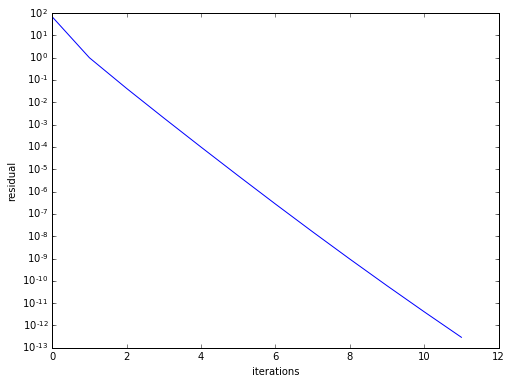
\includegraphics[width=0.5\textwidth]{RS01.PNG}
\caption{AMG, RS coarsening $\theta=0.25$(default), $\epsilon=0.1$}
\end{figure}

\begin{figure}[!htb]
\centering
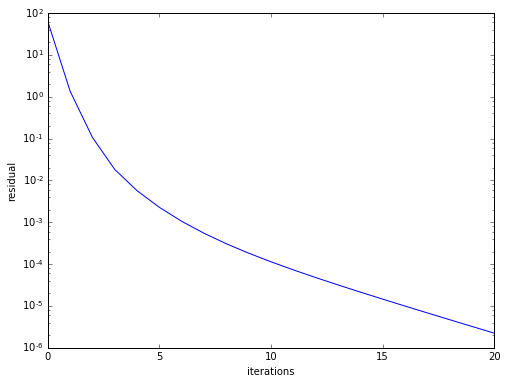
\includegraphics[width=0.5\textwidth]{RS25.PNG}
\caption{AMG, RS coarsening $\theta=0.25$(default), $\epsilon=0.001$, }
\end{figure}

\clearpage 

\section*{Now using $\epsilon=0.001$, try different values for the strength threshold parameter (used to determine the strong connections). How does this change the performance of the solver?}

The setup from the previous question was now tested for a range of strength thresholds $0<\theta<1$ at 0.01 intervals to determine the optimal value for the smallest residual after 20 iterations. Figure 3 plots the residual for the range of thresholds examined. Compared to the default value of 0.25, the optimal value of 0.46 resulted in a residual nearly three orders of magnitude lower. The optimized convergence factor is now (incidentally) 0.46. Interestingly, the optimal value is rather ``brittle'' in that increasing by just 0.01 to 0.47 resulted in a huge jump in the residual to a final value even worse than the one resulting from the default value of the threshold.

The performance of the solver is almost unchanged using the optimal value of the strength threshold compared to the default value; Figure 4 compares the tabulated diagnostic data for each case. The optimal threshold leads to an increased number of levels in the hierarchy, but the relative asymptotic work of the optimal case converges to nearly the same value as the default case.
\begin{figure}[!htb]
\centering
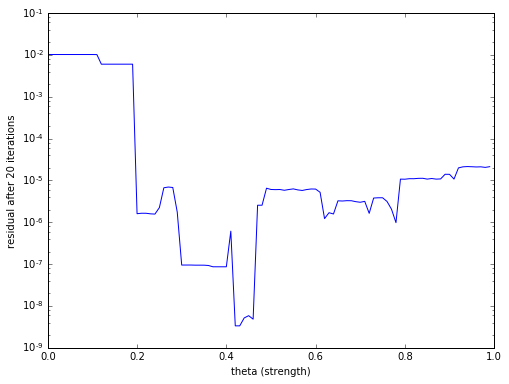
\includegraphics[width=0.6\textwidth]{RS.PNG}
\caption{Behavior of residual after 20 iterations for a range of strength threshold values for RS coarsening.}
\end{figure}

\begin{figure}[!htb]
\centering
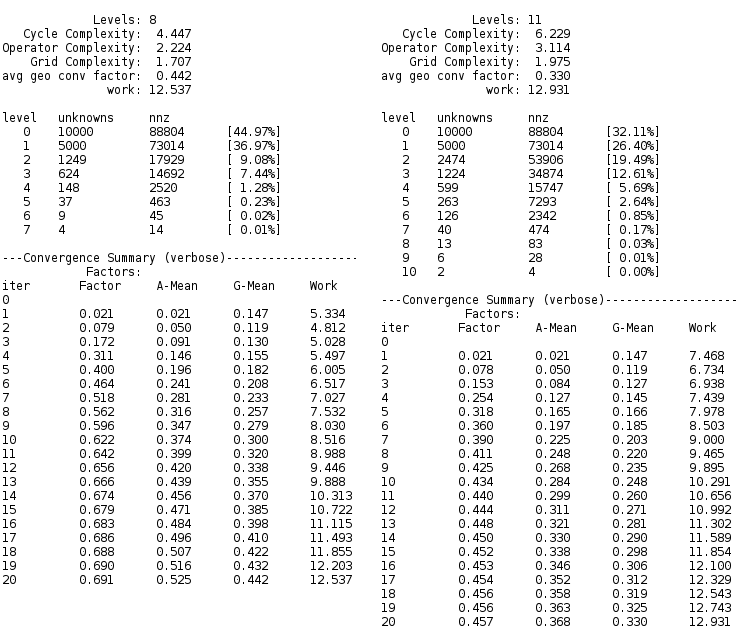
\includegraphics[width=0.9\textwidth]{RS2546tab.PNG}
\caption{Comparison of performance of default(left) and optimal(right) strength thresholds RS coarsening.}
\end{figure}

\clearpage

\section*{Finally, consider two different types of coarsening: Ruge-Stuben (RS) and Cleary-Luby-Jones-Plassmann (CLJP). Assess the cost of the resulting problem at each level for these coarsening algorithms (you may want to look at the number of non-zeros and size of the problem for each level). Solve the anisotropic, rotated diffusion problem with AMG solvers using RS and CLJP coarsening and compare the performance of the solver in each case.}

We can perform a similiar procedure for CLJP coarsening to determine the optimal strength threshold for comparison purposes, with the results plotted in Figure 5. In this case the optimal threshold was 0.36, but notably the optimal value isn't nearly as sensitive as it was in the RS coarsening cases. Additionally the optimal CLJP coarsening results in a much larger residual after 20 iterations compared to RS coarsening as demonstrated in the plots of Figure 6 which shows the evolution of the residual for both coarsening methods. In the optimal threshold CLJP case the asymptotic convergence factor was 0.66 compared to the RS convergence factor of 0.46.

We can now compare the performance of the solver resulting from the two coarsening methods. Figure 7 plots the tabulated data for each method with optimized threshold value. We can see in this case not only does CLJP have a worse residual after a fixed number of iterations and worse convergence factor, but the relative work and sparsity of some coarser levels is worse as well. For instance compare the number of non-zeros for the first several levels; in the CLJP case the number of non-zeros actually remains relatively unchanged across the three levels, despite the number of unknowns decreasing. Level 2 for the CLJP case has nearly 10 times the density of non-zeros as the fine level, to be fair however the density of the RS case at level 2 is 4.4 times that of the fine level (though still not as bad as CLJP). A final performance comparison can be made regarding the asymptotic relative work, with the CLJP case nearly double that of the RS case.

\begin{figure}[!htb]
\centering
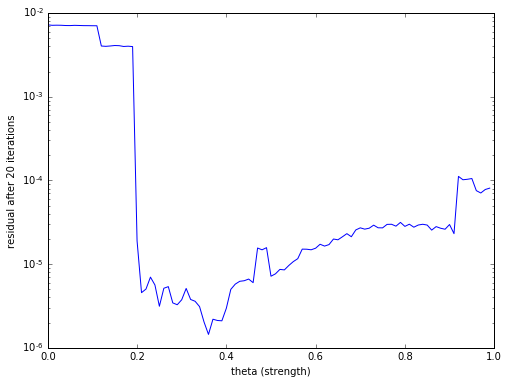
\includegraphics[width=0.5\textwidth]{CLJP.PNG}
\caption{Behavior of residual after 20 iterations for a range of strength threshold values for CLJP coarsening.}
\end{figure}

\begin{figure}[!htb]
\centering
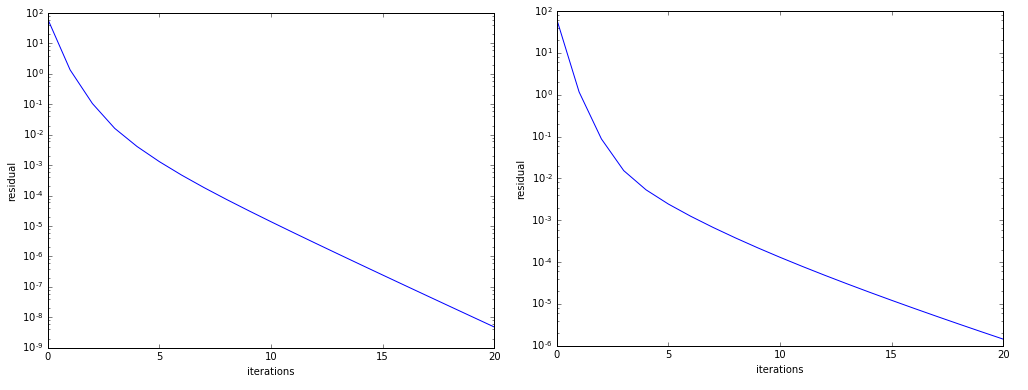
\includegraphics[width=0.8\textwidth]{RS46CLJP36.PNG}
\caption{Comparison of evolution of residual for optimal threshold cases for RS(left) and CLJP(right) coarsening.}
\end{figure}

\begin{figure}[!htb]
\centering
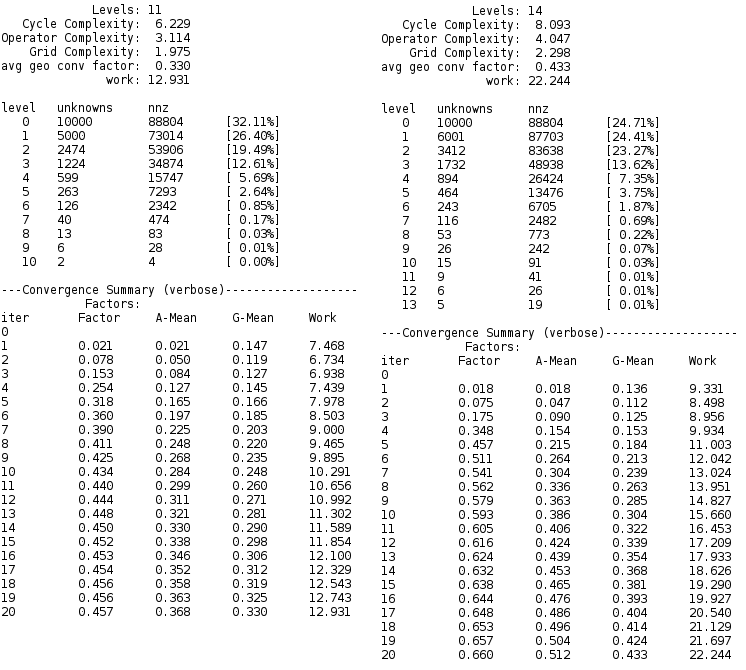
\includegraphics[width=1\textwidth]{RS46CLJP36tab.PNG}
\caption{Comparison of cost at each level for the two optimal threshold coarsening methods, RS(left) and CLJP(right).}
\end{figure}

\end{document}
